\section{问题一的模型的建立和求解}
\subsection{问题一的描述与分析}
\begin{figure}[htbp]
    \centering
    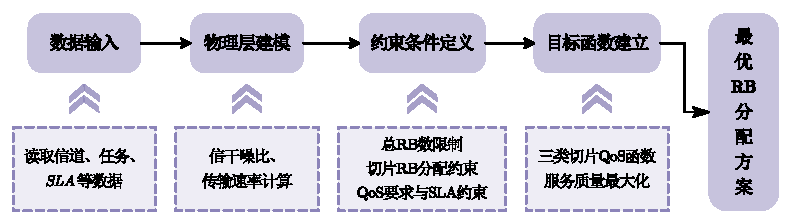
\includegraphics[width=0.85\textwidth]{figures/第一问分析.pdf}
    \caption{问题一场景与资源分配分析示意图}
    \label{fig:q1-analysis}
\end{figure}

问题一考虑单个微基站的资源分配场景。该基站拥有50个资源块(Resource Block, RB),需要为三类网络切片——URLLC(高可靠低时延)、eMBB(增强移动宽带)和mMTC(大规模机器通信)进行资源分配,以最大化用户服务质量。这是一个静态资源分配优化问题,需要在满足资源约束的条件下,找到最优的资源块分配方案。

\subsection{预备工作}
\subsubsection{关键参数补充}

\textbf{基站与信号参数}:基站发射功率 $p_{\text{tx}} = 30$ dBm,单个资源块(RB)带宽 $b = 360$ kHz,噪声系数 $NF = 7$ dB。

\textbf{决策周期}:系统每 $T_{\text{window}} = 100$ ms进行一次资源分配决策。

\textbf{切片资源占用与服务等级协议(SLA)}:URLLC切片:每个用户占用10个资源块,要求时延 $L_k^U \leq 5$ ms,速率 $r_k \geq 10$ Mbps;
eMBB切片:每个用户占用5个资源块,要求时延 $L_k^e \leq 100$ ms 且传输速率 $r_k \geq 50$ Mbps;
mMTC切片:每个用户占用2个资源块,要求时延 $L_k^m \leq 500$ ms,速率 $r_k \geq 1$ Mbps。


\textbf{QoS评估参数}:U切片的效益折扣系数 $\alpha = 0.95$,任务丢失惩罚 $M_U = 5$;e切片的任务丢失惩罚 $M_e = 3$;m切片的任务丢失惩罚 $M_m = 1$。

\subsection{模型建立}

问题一为单时刻静态场景,不引入显式时间索引。每位用户仅有一个任务,服务在一个决策窗口内完成;窗口内允许在各切片内进行“编号靠前优先”的非抢占串并行调度。

\subsubsection{传输速率计算}

根据附录中的信号传输模型,用户$k$占用$i_k$个资源块时的接收功率为:

\begin{equation}
p_{\text{rx},k} = 10^{\frac{p_{\text{tx}} - \phi_k}{10}} \cdot |h_k|^2 \quad \text{(mW)}
\end{equation}
其中,$p_{\text{tx}}$为基站发射功率(dBm),$\phi_k$为大规模衰减(dB),$h_k$为小规模瑞利衰落幅度,$p_{\text{rx},k}$为接收功率(mW)。

考虑噪声功率的影响,噪声功率谱密度为:

\begin{equation}
N_0\big(i_k\big) = -174 + 10\log_{10}\big(i_k \cdot b\big) + 7 \quad \text{(dBm)}
\end{equation}
其中,$i_k$为用户$k$占用的RB数量,$b$为单RB带宽(Hz),$-174$ dBm/Hz为热噪声谱密度,$7$ dB为噪声系数。

信噪比(SNR)为:

\begin{equation}
\gamma_k = \frac{p_{\text{rx},k}}{10^{\frac{N_0\left(i_k\right)}{10}}}
\end{equation}
其中,$N_0(\cdot)$以dBm计,$10^{\frac{N_0\left(i_k\right)}{10}}$为噪声功率(mW)。

根据香农公式,用户$k$的传输速率为:

\begin{equation}
r_k = i_k \cdot b \cdot \log_2\big(1 + \gamma_k\big) \quad \text{(bps)}
\end{equation}
在本问的调度中,同一切片$s\in\{U,e,m\}$内的每位用户占用固定RB数量$v_s$,故$i_k\equiv v_s$。

\subsubsection{时延计算模型}
根据附录中描述的用户任务服务流程,用户的总时延由排队时延和传输时延两部分构成。

用户$k$的传输时延$T_k$为完成其任务数据量$D_k$所需的传输时间:
\begin{equation}
T_k = \frac{D_k \times 10^6}{r_k} \quad \text{(s)}
\end{equation}
其中,$D_k$为任务数据量(Mbit),$r_k$为用户的传输速率(bps)。

给定切片$s$被分配的RB数量$n_s$与每用户占用$v_s$,并发能力为$C_s=\left\lfloor n_s / v_s \right\rfloor$。在同一调度窗口内,切片$s$中的用户按“编号靠前优先”顺序:
初始分配给前$C_s$位用户,其余用户在有会话完成后接续开始服务。由此得到每位用户的等待时延$Q_k$(其开始服务时刻)与传输时延$T_k$,总时延
\begin{equation}
L_k^{s} = Q_k + T_k, \quad s \in \{U, e, m\}.
\end{equation}

\subsubsection{服务质量评估函数}

根据附录中的用户服务质量定义,并结合计算出的总时延,不同切片的QoS评估函数如下:

\textbf{(1) U切片(URLLC)}

服务质量函数为:
\begin{equation}
y_k^{U} = \begin{cases}
\alpha^{L_k^{U}} & \text{若 } L_k^{U} \leq L_{U}^{\text{SLA}} \\
-M_{U} & \text{若 } L_k^{U} > L_{U}^{\text{SLA}}
\end{cases}
\end{equation}
其中,$\alpha\in(0,1)$为效益折扣系数(本题取$\alpha=0.95$),$M_U$为U切片任务丢失惩罚系数,$L_U^{\text{SLA}}$为U切片时延SLA。

\textbf{(2) e切片(eMBB)}

e切片用户采用三段式QoS函数:
\begin{equation}
y_k^{e} = \begin{cases}
1 & \text{若 } r_k \geq r_{e}^{\text{SLA}} \text{ 且 } L_k^{e} \leq L_{e}^{\text{SLA}} \\
\frac{r_k}{r_{e}^{\text{SLA}}} & \text{若 } r_k < r_{e}^{\text{SLA}} \text{ 且 } L_k^{e} \leq L_{e}^{\text{SLA}} \\
-M_{e} & \text{若 } L_k^{e} > L_{e}^{\text{SLA}}
\end{cases}
\end{equation}
其中,$r_e^{\text{SLA}}$、$L_e^{\text{SLA}}$分别为e切片的速率与时延SLA,$M_e$为惩罚系数。

\textbf{(3) m切片(mMTC)}

每个mMTC用户$k$的QoS评估为:
\begin{equation}
y_k^{m} = \begin{cases}
\dfrac{\sum_{i \in \mathcal{U}_{m}} c_i'}{\sum_{i \in \mathcal{U}_{m}} c_i} & \text{若 } L_k^{m} \le L_{m}^{\text{SLA}} \\
-M_{m} & \text{若 } L_k^{m} > L_{m}^{\text{SLA}}
\end{cases}
\end{equation}
其中,$\mathcal{U}_m$为m切片用户集合,$c_i$表示用户$i$是否有任务(本问为“有数据量”),$c_i'$表示该用户是否成功在SLA内完成任务。实现上先计算比例$\text{ratio}=\frac{\sum c_i'}{\sum c_i}$,再对每个有任务的m用户按“成功得$\text{ratio}$,失败得$-M_m$”计分并加总。

\subsubsection{优化模型}

基于上述分析,建立如下单时刻优化模型:

\begin{equation}
\begin{aligned}
\max_{n_U, n_e, n_m} \quad & Q = \sum_{k \in \mathcal{U}_U} y_k^{U} + \sum_{k \in \mathcal{U}_e} y_k^{e} + \sum_{k \in \mathcal{U}_m} y_k^{m} \\
\text{s.t.} \quad & \begin{cases}
 n_U + n_e + n_m = N \\
 n_U \bmod 10 = 0 \\
 n_e \bmod 5 = 0 \\
 n_m \bmod 2 = 0 \\
 n_s \in \mathbb{Z}_{\ge 0}, \quad \forall s \in \mathcal{S}
 \end{cases}
 \end{aligned}
 \end{equation}
其中,$n_U, n_e, n_m$分别为分配给U、e、m切片的RB个数,$\mathcal{S}=\{U,e,m\}$,$\mathcal{U}_s$为切片$s$的用户集合。
\subsection{模型求解}

该优化问题属于整数规划问题,考虑到总资源块数量有限($N=50$),且各切片用户占用RB数量固定,使得分配给各切片的RB数量 $n_s(t)$ 的可行组合是有限的。因此,我们采用枚举法结合调度仿真的策略进行求解,以确保找到全局最优解。算法流程如下(本题固定单个决策时刻 $t=t_0$):
\begin{figure}[H]
    \centering
    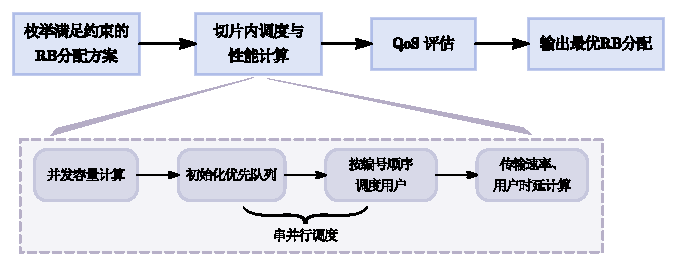
\includegraphics[width=0.85\textwidth]{figures/第一问算法.pdf}
    \caption{第一问资源分配与调度算法流程图}
    \label{fig:q1_algorithm_flow}
\end{figure}

\textbf{Step1:生成RB分配方案}

我们枚举所有满足约束条件的RB分配方案 $(n_U(t), n_e(t), n_m(t))$。为避免资源浪费,分配给各切片的RB数量应为其用户占用量的整数倍。具体地:
\begin{itemize}
    \item $n_U(t)$ 在 $\{0, 10, 20, \dots, 50\}$ 中取值。
    \item $n_e(t)$ 在 $\{0, 5, 10, \dots, 50 - n_U(t)\}$ 中取值。
    \item $n_m(t) = 50 - n_U(t) - n_e(t)$,并检验 $n_m(t)$ 是否为2的倍数。若否则舍弃该方案。
\end{itemize}

\textbf{Step2:切片内调度与性能计算}

对于每一个有效的RB分配方案,我们在各切片内部独立进行调度仿真,以计算每个用户的性能指标。
\begin{itemize}
    \item \textbf{并发容量计算}:对于切片 $s \in \{U, e, m\}$,其并发服务能力为 $C_s = \lfloor n_s(t) / v_s \rfloor$。
    \item \textbf{串并行调度}:在100ms决策周期内,我们采用一种串并行的服务策略。初始时,将前 $C_s$ 个用户(按用户编号排序)分配至并发信道进行传输。当某个用户完成传输后,其占用的信道立即释放,并分配给队列中的下一个用户。
    \item \textbf{性能计算}:通过该调度过程,我们可以计算出每个用户 $k$ 的传输时延 $T_k(t)$ 和等待时延 $Q_k(t)$,从而得到总时延 $L_k(t) = Q_k(t) + T_k(t)$。用户的传输速率 $r_k(t)$ 也一并计算得出。
\end{itemize}

\textbf{Step3:服务质量评估}

根据步骤2计算出的性能指标 $(L_k, r_k)$,我们依据模型中定义的服务质量评估函数计算每个用户的QoS得分 $y_k^s$,并汇总得到当前RB分配方案下的总服务质量 $Q = \sum y_k^s$。

\textbf{Step4:寻找最优方案}

遍历所有RB分配方案后,总服务质量 $Q$ 最高的方案即为问题的最优解。我们记录下最优方案对应的 $(n_U, n_e, n_m)$ 组合、各用户的详细性能指标以及最终的总QoS值。

\subsection{结果分析}
通过执行上述算法,我们得到的最优资源分配方案及对应的性能指标如下:

\textbf{最优资源分配方案}

经枚举计算,我们找到了3个并列的最优资源分配方案,它们均能使系统总服务质量达到最大值15.7823。这三个方案的具体RB分配如下表所示。

\begin{table}[H]
\centering
\caption{并列最优资源分配方案}
\label{tab:q1_best_solutions}
\begin{tabular}{cccccc}
\hline
\textbf{方案} & \textbf{URLLC RB数 ($n_U$)} & \textbf{eMBB RB数 ($n_e$)} & \textbf{mMTC RB数 ($n_m$)} & \textbf{总QoS} \\
\hline
1 & 20 & 10 & 20 & 15.7823 \\
2 & 20 & 20 & 10 & 15.7823 \\
3 & 30 & 10 & 10 & 15.7823 \\
\hline
\end{tabular}
\end{table}

在以上所有方案中,各切片获得的QoS合计分数均相同,分别为:URLLC QoS合计1.9870,eMBB QoS合计3.7953,mMTC QoS合计10.0000。

 这三个方案均实现了资源的高效利用。在实际部署中,可以根据网络运营商的偏好进行选择。例如,方案1(20, 10, 20)为mMTC分配了最多的资源,适合未来mMTC连接数可能增加的场景;方案2(20, 20, 10)则向eMBB倾斜,适合视频流量大的场景;方案3(30, 10, 10)则最优先保障URLLC业务。这些方案共同构成了问题的最优解集。


综上所述,我们提出的资源分配方案能够有效满足各类切片用户的服务需求,实现了系统整体服务质量的最优。